
\de{ĐỀ THI HỌC KỲ I NĂM HỌC 2022-2023}{Sở Giáo Dục Bắc Ninh}
\begin{center}
	\textbf{PHẦN 1 - TRẮC NGHIỆM}
\end{center}
\Opensolutionfile{ans}[ans/ans]

\begin{ex}%[0T3Y1-1]%[Dự án đề kiểm tra HKII NH22-23- Nguyễn Sĩ Đạt]%[SGD Bắc Ninh]
Đồ thị hàm số $y=3 x+2$ đi qua điểm nào?
\choice
{$A(-1 ; 1)$}
{\True $B(1 ; 5)$}
{$C(1 ; 1)$}
{$D(2 ; 0)$}
\loigiai{
\begin{itemize}
\item Với $x=-1$ thay vào ta được $y=3 \cdot (-1)+2=-1$ nên điểm $A$ không thuộc đồ thị.
\item Với $x=1$ thay vào ta được $y=3\cdot1+2=5$ nên điểm $B$ thuộc đồ thị.
\item Với $x=1$ thay vào ta được $y=3 \cdot1+2=5$ nên điểm $C$ không thuộc đồ thị.
\item Với $x=2$ thay vào ta được $y=3 \cdot 2+2=8$ nên điểm $D$ không thuộc đồ thị.
\end{itemize} 
}
\end{ex}

\begin{ex}%[0T3Y1-2]%[Dự án đề kiểm tra HKII NH22-23- Nguyễn Sĩ Đạt]%[SGD Bắc Ninh]
Tập xác định của hàm số $y=\dfrac{1}{x-2}$ là
\choice
{\True $\mathbb{R} \backslash\{2\}$}
{$\{2\}$}
{$(2 ;+\infty)$}
{$(-\infty ; 2)$}
\loigiai{
Điều kiện: $x-2 \ne 0 \Leftrightarrow x \ne 2 $.\\
Vậy tập xác định của hàm số $y=\dfrac{1}{x-2}$ là $\mathbb{R} \backslash\{2\}$.
}
\end{ex}

\begin{ex}%[0T3Y1-1]%[Dự án đề kiểm tra HKII NH22-23- Nguyễn Sĩ Đạt]%[SGD Bắc Ninh]
Cho hàm số $f(x)= \heva{& 2x+1 &\text{ khi } x<1  \\ & \dfrac{1}{x}+3x^2-2 &\text{ khi } x \ge 1 }$. Giá trị của $f(2)$ bằng
\choice
{$\dfrac{31}{2}$}
{$5$}
{\True $\dfrac{21}{2}$} 
{$\dfrac{11}{2}$}
\loigiai{
Ta có $f(2)= \dfrac{1}{2}+3\cdot 2^2 - 2 = \dfrac{21}{2}$.
} 
\end{ex}
\begin{ex}%[0T3B2-1]%[Dự án đề kiểm tra HKII NH22-23- Nguyễn Sĩ Đạt]%[SGD Bắc Ninh]
\immini{Cho hàm số bậc hai $y=f(x)$ có đồ thị như hình vẽ bên. Hàm số trên đồng biến trên khoảng nào?
\choice
{$\left(-\infty; +\infty\right)$}
{$\left(1; +\infty\right)$}
{$\left(0; +\infty\right)$}
{\True $\left(-\infty; 1\right)$}}
{\begin{tikzpicture}[scale=1, line join=round, >=stealth, font=\footnotesize]
		\def\a{-1} % Hệ số a phải khác 0
		\def\b{2}
		\def\c{0}
		\draw[thick,->] (-2,0) -- (4,0) node[below] {$x$};
		\draw[thick,->] (0,-3.5) -- (0,2) node[left] {$y$};
		\draw (0,0)node[below left]{$O$}; 
		\draw[thick,samples=150,smooth,domain=-1:3] plot(\x,{\a*(\x)^2+(\b)*\x+(\c)});
		\foreach \y in {1} 
		{\draw (0.075,\y )--(-0.075,\y) node[left]{$\y$};} 
		\foreach \x in {1} 
		{\draw (\x,0.075 )--(\x,-0.075) node[below]{$\x$};}  
		\draw[dashed] (1,0)|-(0,1);
\end{tikzpicture}}
\loigiai{
Nhìn vào đồ thị, ta thấy hàm số đồng biến trên $\left(-\infty; 1\right)$.
}
\end{ex}

\begin{ex}%[0T3Y2-2]%[Dự án đề kiểm tra HKII NH22-23- Nguyễn Sĩ Đạt]%[SGD Bắc Ninh]
Trong các hàm số sau, hàm số nào là hàm số bậc hai?
\choice
{\True $y=2x^2-3x+2022$}
{$y=-x^2+2x+\dfrac{1}{x}$}
{$y=4-3x$}
{$y=x^2+\sqrt{2x}-x^3$}
\loigiai{
Ta có $y=2x^2-3x+2022$ là hàm số bậc hai.
}
\end{ex}

\begin{ex}%[0T3Y2-3]
Parabol $y=x^2-3x+2$ có trục đối xứng là:
\choice
{\True $x=\dfrac{3}{2}$}
{$x=-\dfrac{3}{2}$}
{$x=3$}
{$x=-3$}
\loigiai{
Parabol $y=x^2-3x+2$ có trục đối xứng là $x=\dfrac{-(-3)}{2}=\dfrac{3}{2}$.
}
\end{ex}

\begin{ex}%[0T3Y2-4] 
Parabol $y=2x^2-3x-2$ cắt trục $Oy$ tại điểm có tọa độ là
\choice
{$\left(-2;0\right)$}
{$\left(-\dfrac{1}{2};0\right)$}
{\True $\left(0;-2\right)$}
{$\left(0;2\right)$}
\loigiai{
Gọi $M\left(x_0;y_0\right)$ là giao điểm của parabol đã cho và trục $Oy$.\\
Vì $M \in Oy$ nên $x_0=0$.\\
Mà $M$ thuộc parabol nên $y_0=2 \cdot 0^2 -3 \cdot 0 -2 =-2$.\\
Vậy $M\left(0;-2\right)$.
}
\end{ex}

\begin{ex}%[0T3B2-2]%[Dự án đề kiểm tra HKII NH22-23- Nguyễn Sĩ Đạt]%[SGD Bắc Ninh]
\immini{Cho hàm số $y=ax^2+bx+c\,\,\left(a,b,c\in\mathbb{R}\right)$ có đồ thị như hình vẽ bên. Mệnh đề nào sau đây đúng?
\choice
{$a>0$, $b>0$, $c>0$}
{$a>0$, $b<0$, $c<0$}
{\True $a>0$, $b<0$, $c>0$}
{$a<0$, $b<0$, $c>0$}}
{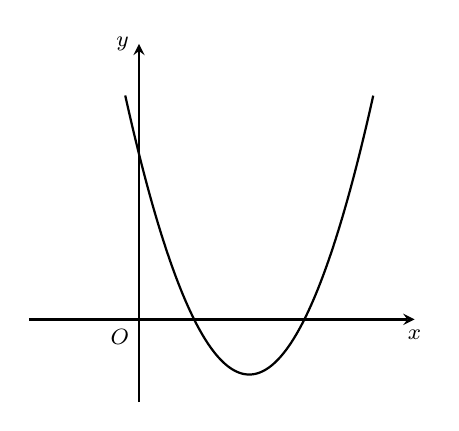
\begin{tikzpicture}[scale=.7, line join=round, >=stealth, font=\footnotesize]
		\def\a{1} % Hệ số a phải khác 0
		\def\b{-4}
		\def\c{3}
		\draw[thick,->] (-2,0) -- (5,0) node[below] {$x$};
		\draw[thick,->] (0,-1.5) -- (0,5) node[left] {$y$};
		\draw (0,0)node[below left]{$O$}; 
		\draw[thick,samples=150,smooth,domain=-.25:4.25] plot(\x,{\a*(\x)^2+(\b)*\x+(\c)});
\end{tikzpicture}}
\loigiai{
Đồ thị hàm số có bề lõm quay lên trên nên $a>0$.\\
Ta lại có giao điểm của đồ thị hàm số với trục tung có tung độ dương nên $c>0$.\\
Mặt khác đỉnh của parabol có hoành độ dương, tức là $\dfrac{-b}{2a}>0$. Mà $a>0$ nên $b<0$.\\
Vậy $a>0$, $b<0$, $c>0$.}
\end{ex}

\begin{ex}%[0T3B2-1]%[Dự án đề kiểm tra HKII NH22-23- Nguyễn Sĩ Đạt]%[SGD Bắc Ninh]%[câu 9]
	Hàm số $y=-2x^2+8x+1$ nghịch biến trên khoảng nào dưới đây?
	\choice
	{$(-\infty;2)$}
	{$(-2;+\infty)$}
	{\True $(2;+\infty)$}
	{$(-\infty;-2)$}
	\loigiai{
	Điểm $S(2;9)$ là đỉnh của hàm số $y=-2x^2+8x+1$.\\
	Vì hàm số bậc hai có $a=-2<0$ nên ta có bảng biến thiên sau:
	\begin{center}
		
\begin{tikzpicture}[>=stealth,x=1cm,y=1cm,scale=1]
		\tkzTabInit[lgt=1.5,espcl=3,deltacl=1]{$x$/1 ,$y$/2}
		{$-\infty$ , $2$ , $+\infty$}
		\tkzTabVar{-/$-\infty$ , +/$9$ , -/$-\infty$}
		\end{tikzpicture}
	\end{center}
	Vậy hàm số $y=-2x^2+8x+1$ nghịch biến trên $(2;+\infty)$.
	}
\end{ex}
\begin{ex}%[0T5Y2-2]%[Dự án đề kiểm tra HKII NH22-23- Nguyễn Sĩ Đạt]%[SGD Bắc Ninh]%câu 10
	Cho tam giác $ABC$ có $I$ là trung điểm $AB$. Mệnh đề nào sau đây đúng?
	\choice
	{\True$\vec{CA}+\vec{CB}=2\vec{CI}$}
	{$\vec{CI}+\vec{CB}=2\vec{CA}$}
	{$\vec{CA}+\vec{CI}=2\vec{CB}$}
	{$\vec{CA}-\vec{CB}=2\vec{CI}$}	
	\loigiai{
		$I$ là trung điểm $AB$ nên $\vec{CA}+\vec{CB}=2\vec{CI}$.
	}
\end{ex}
\begin{ex}%[0T5Y2-2]%[Dự án đề kiểm tra HKII NH22-23- Nguyễn Sĩ Đạt]%[SGD Bắc Ninh]
	Cho tam giác $ABC$ có $I$ là trung điểm $AB$. Mệnh đề nào sau đây đúng?
	\choice
	{$\vec{MA}+\vec{MB}+\vec{MC}=3\vec{GM}$}
	{\True$\vec{MA}+\vec{MB}+\vec{MC}=3\vec{MG}$}
	{$\vec{MA}+\vec{MB}+\vec{MC}=\vec{MG}$}
	{$\vec{MA}+\vec{MB}+\vec{MC}=\vec{0}$}	
	\loigiai{
		$G$ là trọng tâm của tam giác $ABC$ nên $\vec{MA}+\vec{MB}+\vec{MC}=3\vec{MG}$.
	}
\end{ex}

\begin{ex}%[0T5B3-1]%[Dự án đề kiểm tra HKII NH22-23- Nguyễn Sĩ Đạt]%[SGD Bắc Ninh]
Một con tàu chở hàng $A$ đang đi từ hướng đông sang tây với tốc độ $20$ hải lí/giờ. Cùng lúc đó, một con tàu chở khách $B$ đang đi từ hướng tây sang hướng đông với tốc độ $40$ hải lí/giờ. Gọi $\vec{a}$, $\vec{b}$ lần lượt là các vectơ vận tốc của tàu $A$ và tàu $B$. Biết rằng $\vec{b}=k\cdot\vec{a}$, giá trị của $k$ bằng
	\choice
	{$\dfrac{1}{2}$}
	{$-\dfrac{1}{2}$}
	{$2$}
	{\True $-2$}	
	\loigiai{
Ta có $\vec{a}$ ngược hướng $\vec{b}$ và $\left| \vec{b}\right|=2\cdot \left| \vec{a}\right|$.\\
Suy ra $\vec{b}=-2\cdot\vec{a}$.
	}
\end{ex}

\Closesolutionfile{ans}
%\begin{center}
%	\textbf{ĐÁP ÁN}
%	\inputansbox{10}{ans/ans}	
%\end{center}
\begin{center}
	\textbf{PHẦN 2 - TỰ LUẬN}
\end{center}


\begin{bt}%[0D3B1-2] %[Dự án đề kiểm tra HKI NH22-23- Nguyễn Ngọc Nguyên]%[Sở GD & ĐT Bắc Ninh]
Tìm tập xác định của các hàm số sau
	\begin{listEX}[3]
		\item $y=\dfrac{3x+5}{6-2x}$;
		\item $y=\sqrt{x-1}$;
		\item $y=\dfrac{1}{x}+\sqrt{3-x}$.
	\end{listEX}
\loigiai{
\begin{listEX}
	\item Hàm số $y=\dfrac{3x+5}{6-2x}$ xác định khi và chỉ khi $6-2x \ne 0 \Leftrightarrow x \ne 3$. \\
	Tập xác định của hàm số là $\mathscr{D}=\mathbb{R} \setminus \{3\}$.
	\item Hàm số $y=\sqrt{x-1}$ xác định khi và chỉ khi $x-1 \ge 0 \Leftrightarrow x \ge 1$.\\
	Tập xác định của hàm số là $\mathscr{D}=[1;+\infty)$.
	\item Hàm số $y=\dfrac{1}{x}+\sqrt{3-x}$ xác định khi và chỉ khi $\heva{&x \ne 0 \\ & 3-x \ge 0} \Leftrightarrow \heva{&x\ne 0 \\ &x \le 3.}$\\
	Tập xác định của hàm số là $\mathscr{D}=(-\infty;3] \setminus \{0\}$.
\end{listEX}
}
\end{bt}

\begin{bt}%[0D3K2-1]%[0D3B2-3]%[Dự án đề kiểm tra HKI NH22-23- Nguyễn Ngọc Nguyên]%[Sở GD & ĐT Bắc Ninh]
	\begin{enumerate}
		\item Cho hàm số $y=x^2+bx+c$ có đồ thị là parabol $(P)$. Tìm hàm số trên biết $(P)$ đi qua điểm $A(0;6)$ và có trục đối xứng là $x=1$.
		\item Tìm các khoảng đồng biến, nghịch biến và vẽ đồ thị hàm số $y=-x^2+4x$.
	\end{enumerate}
	\loigiai{
\begin{enumerate}
	\item Đồ thị hàm số $y=x^2+bx+c$ đi qua điểm $A(0;6)$ và có trục đối xứng $x=1$ nên ta có hệ phương trình $\heva{&c=6 \\ &-\dfrac{b}{2}=1} \Leftrightarrow \heva{&c=6 \\ &b=-2.}$\\
	Vậy hàm số là $y=x^2-2x+6$.
	\item 
	\begin{itemize}
		\item Tập xác định $\mathscr{D}=\mathbb{R}$.
		\item Tọa độ đỉnh $I=(2;4)$.
		\item Trục đối xứng $x=2$.
		\item Hàm số đồng biến trên khoảng $(-\infty;2)$ và nghịch biến trên khoảng $(2;+\infty)$.
		\item Hệ số $a=-1<0$ nên đồ thị hàm số $y=-x^2+4x$ là một parabol có bề lõm hướng xuống dưới.
		\item Đồ thị cắt $Oy$ tại điểm $O(0;0)$, cắt $Ox$ tại $O(0;0)$ và $A(4;0)$.
	\end{itemize}
\begin{center}
	\begin{tikzpicture}[scale=0.85,>=stealth, font=\footnotesize, line join=round, line cap=round]
		\def\xmin{-1} \def\xmax{5}
		\def\ymin{-1} \def\ymax{5} 
		\draw[->] (\xmin,0)--(\xmax,0) node [below]{$x$};
		\draw[->] (0,\ymin)--(0,\ymax) node [left]{$y$};
		\node at (0,0) [below left]{$O$};
		\clip (\xmin+0.1,\ymin+0.1) rectangle (\xmax-0.5,\ymax-0.1);
		\draw[smooth,samples=300,domain=-0.5:4.5] plot(\x,{-(\x)^2+4*(\x)});
		\node at (0,4)[above left ]{$4$};
		\node at (2,0) [below left]{$2$};
		\node at (4,0) [below left]{$4$};
		\draw[dashed] (0,4)--(2,4)--(2,0);
	\end{tikzpicture}
\end{center}
\end{enumerate}	
}
\end{bt}



\begin{bt}%[0H2B3-2]%[0H2B3-3]%[0H2K3-8]%[Dự án đề kiểm tra HKII NH22-23- Võ Thị Thùy Trang]%[Sở Bắc Ninh]
		Cho tam giác $ABC$ đều có độ dài cạnh bằng $a$. Gọi $N$ là trung điểm $BC$ và $M$ là điểm thay đổi trên đường thẳng $AC$.
	\begin{enumerate}
		\item Chứng minh $\overrightarrow{AB}+2 \overrightarrow{BN}=\overrightarrow{AC}$.
		\item Xác định vị trí điểm $I$ sao cho $\overrightarrow{IA}-\overrightarrow{IB}+\overrightarrow{IC}=\overrightarrow{0}$.
		\item Tìm giá trị nhỏ nhất của biểu thức $P=\left|\overrightarrow{MA}+\overrightarrow{M B}+\overrightarrow{M C}\right|+3\left|\overrightarrow{MA}-\overrightarrow{MB}+\overrightarrow{MC}\right|$.
	\end{enumerate}
\loigiai{\immini{\begin{enumerate}
			\item Ta có $\overrightarrow{AB}+2 \overrightarrow{BN}=\overrightarrow{AB}+\overrightarrow{BC}=\overrightarrow{AC}$.
			\item  $\overrightarrow{IA}-\overrightarrow{IB}+\overrightarrow{IC}=\overrightarrow{0} \Leftrightarrow \overrightarrow{BA}+\overrightarrow{IC}=\overrightarrow{0} \Leftrightarrow \overrightarrow{BA}=\overrightarrow{CI}$.\\
			Do đó $I$ là đỉnh của hình bình hành $AICB$.
			\item Gọi $G$ là trọng tâm của tam giác $ABC$.\\ Khi đó $\overrightarrow{MA}+\overrightarrow{MB}+\overrightarrow{MC}=3\overrightarrow{MG}$.\\
			$\overrightarrow{MA}-\overrightarrow{MB}+\overrightarrow{MC}=\overrightarrow{BA}+\overrightarrow{MC}=\overrightarrow{CI}+\overrightarrow{MC}=\overrightarrow{MI}$.
	\end{enumerate}}
{	\begin{tikzpicture}[scale=0.7, font=\footnotesize, line join=round, line cap=round, >=stealth]
		\def\bc{4} % cạnh BC
		\def\ba{4} % cạnh BA
		\def\h{4} % đường cao
		\def\gocB{60} % góc B của đáy
		\coordinate[label=below left:$B$] (B) at (0,0);
		\coordinate[label=above:$A$] (A) at (\gocB:\ba);
		\coordinate[label=right:$C$] (C) at (\bc,0);
		\coordinate[label=below:$N$] (N) at ($(C)!0.5!(B)$);
		\coordinate[label=above:$I$] (I) at ($(A)+(C)-(B)$);
		\coordinate[label=left:$G$] (G) at ($(A)!2/3!(N)$);
		\coordinate[label=below:$M$] (M) at ($(A)!1.5!(C)$);
		\draw (A)--(B)--(C)--(A) (C)--(I) (A)--(N) (C)--(M);
		\draw (M)--(I)--(G)--(M) (G)--(C);
		\pic[draw,angle radius=2mm,angle eccentricity=3] { right angle = G--C--I};
		\foreach \diem in {A,B,C,N,I,G,M}	\fill (\diem)circle(1.5pt);
\end{tikzpicture}}
$P=\left|\overrightarrow{MA}+\overrightarrow{MB}+\overrightarrow{MC}\right|+3\left|\overrightarrow{MA}-\overrightarrow{MB}+\overrightarrow{MC}\right|=3MG+3MI=3\left(MG+MI\right)\ge 3GI$.\\
Tam giác $CGI$ vuông tại $C$ nên $GI=\sqrt{CG^2+CI^2}=\sqrt{\dfrac{a^2}{3}+a^2}=\dfrac{2a\sqrt{3}}{3}$.\\
Vậy giá trị nhỏ nhất của $P$ bằng $2a\sqrt{3}$ khi $M=CA\cap GI$.
}
\end{bt}
\begin{bt}%[0D3B1-1]%[0D3B1-3]%[Dự án đề kiểm tra HKII NH22-23- Võ Thị Thùy Trang]%[Sở Bắc Ninh]
	Bác A thường xuyên phải đi công tác bằng taxi với quãng đường trên $20 \mathrm{~km}$. Bác liên hệ với một hãng taxi và nhận được thông báo giá cước (đã bao gồm thuế VAT) như sau
	\begin{center}
		\begin{tabular}{|c|c|c|c|}
			\hline Quãng đường $x$(km) & $0<x \leq 0,5$ & $0,5<x \leq 20$ & $x>20$ \\
			\hline Giá cước & 10000 đồng & 14100 đồng $/ 1\mathrm{~km}$ & 12300 đồng/$ 1\mathrm{km}$ \\
			\hline
		\end{tabular}
	\end{center}
	\begin{enumerate}
		\item Lập công thức tính số tiền mà bác A phải trả theo $x$.
		\item Nếu bác A đi $25 \mathrm{~km}$ thì bác A phải trả bao nhiêu tiền?
	\end{enumerate}
	\loigiai{
		\begin{enumerate}
		\item Gọi $x$ là số kilômét bác A di chuyển $(x>0)$.\\
		Khi đã lên taxi đi bác A luôn phải trả $10000$ đồng dù đi hay không, do đó số tiền phải trả luôn bao gồm $10000$ đồng này.
		    \begin{itemize}
		    	\item Nếu $0 \leq x \le 0{,}5$, số tiền phải trả là 10000 đồng.
		    	\item Nếu $0{,}5<x \le 20$, số tiền phải trả là
		    	$10000+14100(x-0{,}5)=2950+14100x$.
		    	\item Nếu $x>20$, số tiền phải trả là
		    	$$10000+14100\cdot(20-0{,}5)+12300(x-20)=38950+12300x.$$
		    \end{itemize}
	    Vậy hàm số $f(x)$ có công thức $f(x)=\heva{&10000 &&\text{Với}~ 0 \leq x \le 0{,}5\\&2950+14100x &&\text{Với}~0{,}5<x \le 20\\&38950+12300x &&\text{Với}~x>20.}$   
		\item Nếu bác A đi $25 \mathrm{~km}$ thì bác A phải trả số tiền là\\ $f(25)=38950+12300\cdot 25=346450$ đồng.
	\end{enumerate}
}
\end{bt}
